\newcommand{\assignmentDate}{November 4th, 2019}

% Add title
%Institute
\begin{tabular*}{\hsize}{l@{\extracolsep{\fill}} r}
	\textsc{Technical University of Berlin}		 \hfill&								 	\\
	Faculty II - Mathematics and Natural Sciences\hfill&									\\
	Institute of Mathematics 					 \hfill&									\\
	Dr. D. Peschka, A. Selahi 		 			 \hfill&									\\
\end{tabular*}

% Title
\begin{center}
	\textbf{\Large{\courseName}}\\
	\vspace{7pt}
	\large{Homework \currentAssignment}\\
	\smallskip
	\normalsize{Submitted on \assignmentDate}
\end{center}

% Group table
\begin{center}
	\vspace{-8pt}
	\begin{tabular}{l c r}
		by \textbf{\groupNumber}		    &	 			  &		 								\\
		\hline
		\texttt{Kagan Atci} 			    & \texttt{338131} & \texttt{Physical Engineering, M.Sc.}\\
		\texttt{Navneet Singh }		 	    & \texttt{380443} & \texttt{Scientific Computing, M.Sc.}\\ 
		\texttt{Daniel V. Herrmannsdoerfer} & \texttt{412543} & \texttt{Scientific Computing, M.Sc.}\\ 
		\hline
	\end{tabular}
\end{center}


% EXERCISE 1
% --------------------------------------------------------------------------------------------------------------------
\addExercise{1}{Ex1}
Given is the following boundary problem of an annulus
\begin{equation}
	\begin{cases}
		-\Delta u = 0, &\text{in } \Omega = \{(x,y) \in \mathbb{R}^2 \colon 1 \leq \sqrt{x^2 + y^2} < 2 \} \subset \mathbb{R}^2, \\
		u = g, &\text{on } \partial \Omega,
	\end{cases}
	\label{eq:annulus1}
\end{equation}
with the boundary condition
\begin{equation}
	g(x,y) = 
	\begin{cases}
		x &\text{for } x^2 +y^2 = 2^2\\
		0 &\text{otherwise}
	\end{cases}
\end{equation}
%
% ----------------
\addSubExercise{a}
$(x,y) \in \Omega$ is transformed to polar coordinates $(r, \varphi) \in \Omega_r$ using
\begin{align}
	x &= r \cos{(\varphi)},\\
	y &= r \sin{(\varphi)}
\end{align}
with $r \in (1,2]$ and $\varphi \in (0, 2 \pi]$. Let $v:\Omega_r \to \mathbb{R}$ defined by $v(r,\varphi) = v(x,y)$.
In this case, the partial derivatives $v_x$ and $v_y$ are expressed using chain rule as follows
\begin{align}
	%\frac{}{}
	\label{eq:chainX}
	\frac{\partial v}{\partial x} &= \frac{\partial v}{\partial r} \frac{\partial r}{\partial x} +
									\frac{\partial v}{\partial \varphi} \frac{\partial \varphi}{\partial x}, \text{also denoted as } u_x = u_r r_x + v_\varphi \varphi_x\\
	%
	\label{eq:chainY}
	\frac{\partial v}{\partial x} &= \frac{\partial v}{\partial r} \frac{\partial r}{\partial x} +
									\frac{\partial v}{\partial \varphi} \frac{\partial \varphi}{\partial x}, \text{also denoted as } u_y= u_r r_y + v_\varphi \varphi_y
\end{align}
%
The second partial derivative of $v$ with respect to $x$ is obtained using product rule
\begin{equation}
	v_{xx} = u_r r_{xx} + (u_r)_x r_x + v_\varphi \varphi_{xx} + (v_\varphi)_x \varphi_x
	\label{eq:uXX}
\end{equation}
%
By applying the chain rule from \EQ{chainX} and \EQ{chainY} into  \EQ{uXX}, $v_{xx}$ is written in the following form
%
\begin{equation}
	v_{xx} = u_r r_{xx} + v_{rr} r_{x}^2 + 2 v_{r\varphi} r_x \varphi_x + v_\varphi \varphi_{xx} + v_{\varphi \varphi} \varphi_x^2
	\label{eq:uXX_chain}
\end{equation}
%
where a similar expression is obtained for y
\begin{equation}
	v_{yy} = u_r r_{yy} + v_{rr} r_{y}^2 + 2 v_{r\varphi} r_y \varphi_y + v_\varphi \varphi_{yy} + v_{\varphi \varphi} \varphi_y^2
	\label{eq:uYY_chain}
\end{equation}
%
The laplace equation $\Delta v = v_{xx} + v_{yy}$ can be written in a proper semi-polar coordinate form by adding \EQ{uXX_chain} and \EQ{uYY_chain} and collecting the like terms
\begin{align}
	\nonumber
	\Delta v &= v_{xx} + v_{yy}\\
	\label{eq:laplaceExpanded}
			 &= u_r(r_{xx} + r_{yy}) + v_{rr} (r_x^2 + r_y^2) + 2 v_{r\varphi} (r_x \varphi_{x} + r_y \varphi_y) + v_\varphi (\varphi_{xx} + \varphi_{yy}) + v_{\varphi\varphi} (\varphi_x^2 + \varphi_y^2)
\end{align}
%
Now, expressions in parentheses are to be elaborated in the partial derivations with respect to polar coordinates.
For this purpose, the relationship $x^2 + y^2 = r^2$ is differentiated with respect to x and y.
Accordingly, the partial differentiation of $r$ terms with respect Cartesian terms up to second order are obtained as
\begin{align}
	\label{eq:r_x}	
	r_x    &= \frac{x}{r},\\
	r_{xx} &= \frac{y^2}{r^3},\\
	r_{y}  &= \frac{y}{r},\\
	r_{yy} &= \frac{x^2}{r^3}\text{.}
\end{align}
%
Similarly, the partial differentiation of $\varphi$ terms with respect to x and y are obtained as
\begin{align}
	\varphi_x    &= -\frac{y}{r^2},\\
	\varphi_{xx} &= \frac{2xy}{r^4},\\
	\varphi_{y}  &= \frac{x}{r^2},\\
	\label{eq:phi_yy}
	\varphi_{yy} &= -\frac{2xy}{r^4}\text{.}
\end{align}
%
Employing the Equations \ref{eq:r_x} to \ref{eq:phi_yy} in \EQ{laplaceExpanded} gives
\begin{align*}
	\Delta v &= u_r\left(\frac{y^2}{r^3} + \frac{x^2}{r^3}\right) + v_{rr} \left(\left(\frac{x}{r} \right)^2+ \left(\frac{y}{r} \right)^2\right) + 2 v_{r\varphi} \left(\frac{-xy}{r^3}+\frac{yx}{r^3}\right) + \hdots\\
			 &v_\varphi \left(\frac{2xy}{r^4} - \frac{2xy}{r^4}\right) + v_{\varphi\varphi} \left(\left(-\frac{x^2}{r^3}\right) ^2 + \left(\frac{x^2}{r^3}\right)^2 \right)\\
			 &= \frac{1}{r} u_r + v_{rr} + 0 + 0 + \frac{1}{r^2} v_{\varphi\varphi}.
\end{align*}
Thus, for any $v$ satisfying the Laplace equation $-\Delta v = 0$, $v$ satisfies in polar coordinates the equation
\begin{equation}
	\label{eq:laplacePolar}
	-\left(v_{rr} + \frac{1}{r} v_r + \frac{1}{r^2} v_{\varphi\varphi}\right)=0
\end{equation}
%
% ----------------
\addSubExercise{b}
For any $v$ defined in a), the domain $\Omega_v$ is defined as
\begin{equation}
	\Omega_v = \{(r,\varphi) \in \mathbb{R}^2 \colon r \in (1,2), \varphi \in (0, 2\pi]\}
\end{equation}
with the boundary condition 
\begin{equation}
	\label{eq:boundaryPolar}
	h(r, \varphi) =
	\begin{cases}
		2\cos{(\varphi)} &\text{ for } r = 2,  \varphi \in (0, 2\pi] \\
		0 &\text{otherwise}
	\end{cases}
\end{equation}
%
% ----------------
\newcommand{\constFac}{\lambda}
\addSubExercise{c}
Assuming that $v(r,\varphi) = R(r)\Phi(\varphi) \text{, } \forall r \in (0,1] \text{, } \forall \varphi \in (0,2\pi]$.
If $v(r,\varphi)$ satisfies \EQ{laplacePolar}, then this equation can be expressed in the following form
\begin{equation}
	\label{eq:laplaceSep}
	\left(R_{rr} \Phi + \frac{1}{r} R_r \Phi + \frac{R}{r^2} \Phi_{\varphi\varphi}\right) = 0
	\text{.}
\end{equation}
Placing the functions depended of $r$ and $\varphi$ in separate terms, \EQ{laplaceSep} is written as
\begin{equation}
	\label{eq:laplaceSep2}
	-\frac{r^2 R_{rr} + r R_r}{R} = \frac{\Phi_{\varphi\varphi}}{\Phi} = \constFac
\end{equation}
where $\constFac$ represent a constant real factor.
\EQ{laplaceSep2} enables $v(r,\varphi)$ to be considered as two different ODE's, as both $R$ and $\Phi$ terms are equated with $\constFac$ separately
%
\begin{align}
	\label{eq:odePhi}
	\frac{\Phi_{\varphi\varphi}}{\Phi} &= \constFac \iff    \Phi_{\varphi\varphi} = \Phi \constFac \\ 
	\label{eq:odeR}
	-\frac{r^2 R_{rr} + r R_r}{R} &= \constFac      \iff   -\left(r^2 R_{rr} + r R_r \right) = R \constFac
	\text{.}
\end{align}
%
% ----------------
\addSubExercise{d}
The solution of $v(r,\varphi)$ consists of the superposition of \EQ{odePhi} and \EQ{odeR} solutions, which are studied in three different cases for $\lambda$:
\begin{itemize}
	\item {\boldmath$\lambda = 0$}: \\
		In this case, possible solutions are given by\\
		\begin{align}
			\Phi(\varphi)&= a \varphi + b\\
			R(r)         &= c \ln{r} + d
			\text{.}
		\end{align}
		Since $\Phi$ has to be a periodic equation, $a = 0$, and $c = 0$, as the solution has to remain finite, as $r$ goes to 0.
		With the applied conditions, the ansatz gives
		\begin{equation}
			\label{eq:vLambda1}
			v(r, \varphi) = b d = g = const.
		\end{equation}
%
	\item {\boldmath$\lambda < 0$}: \\
		Let $\lambda = -k^2$.
		Possible solutions for $R$ and $\Phi$ are given by
		\begin{align}
		\label{eq:phiLambda2}
			\Phi(\varphi)&= a_k \cosh{(k\varphi)} + b_k \sinh{(k\varphi)}\\
			R(r)         &= c_k r^{-k} + d_k r^{k}
		\end{align}
		$v(r,\varphi)$ holds no solutions for this case, because \EQ{phiLambda2} implies a periodic function in neither terms, thus remains zero for $\Phi$.
%
	\item {\boldmath$\lambda > 0$}: \\
		Let $\lambda = k^2$.
		Possible solutions are given by
		\begin{align}
		\label{eq:phiLambda3}
			\Phi(\varphi)&= a_k \cos{(k\varphi)} + b_k \sinh{(k\varphi)}\\
			R(r)         &= c_k r^{k} + d_k r^{-k}
		\end{align}
		In this case, $\Phi$ shows a well periodic function with period $2\pi$.
		Furthermore $d_k$ must be 0, in order to keep $R$ finite, as $r$ goes to zero
		\begin{equation}
		\label{eq:vLambda3}
			v(r, \varphi) = r^k \left( A_k \cos{(k \varphi)} + B_k \sin(k \varphi)\right)
		\end{equation}
		where $A_k = a_k c_k$ and $B_k = b_k c_k$.
\end{itemize}
The solution for $v(r, \varphi)$ is expressed as the superposition of \EQ{vLambda1} and \EQ{vLambda3}
\begin{equation}
	v(r, \varphi) = g + \sum_{k=1}^{} r^k \left( A_k \cos{(k \varphi)} + B_k \sin(k \varphi)\right)
\end{equation}
for $A_k$ and $B_k \in \mathbb{R}$ are obtained by the Fourier expansion.
\par
The solution of $v(r, \varphi)$ is to be investigated on the boundary with $r = 2$.
So gives
\begin{equation}
	\label{eq:vBoundary}
	v(2, \varphi) = g + \sum_{k=1}^{} 2^k \left( A_k \cos{(k \varphi)} + B_k \sin(k \varphi)\right)
\end{equation}
As \EQ{vBoundary} implies, the boundary condition is already given in the Fourier-series form, so that the only solution exists for $k = 1$, $A_1 = 0$, $B_1 = 0$ and $g=0$.
Hence the solution, that satisfies \EQ{laplacePolar} and \EQ{boundaryPolar} in $\Omega_v$ is
\begin{equation}
	\label{eq:vSol}
	v(r, \varphi) = r \cos{(\varphi)}
	\text{.}
\end{equation}
%
% ----------------
\addSubExercise{e \& f}
The solution code can be found in \texttt{a02e01solution.m} and the plot code in \texttt{a02e01plot.m}.
The surface plot of the \EQ{vSol} solution is illustrated in \FIG{a02e01plot}.
\begin{figure}[H]
\vspace*{\FigUpperVSpace}
\def\MeshFigWidth{220pt}
	\begin{subfigure}{0.5\hsize}
		\centering
		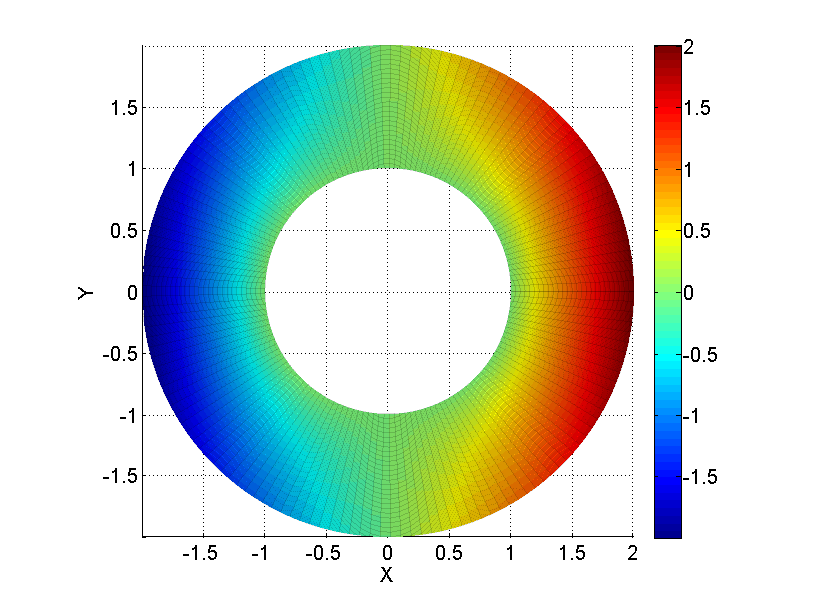
\includegraphics[width=\MeshFigWidth]{a02e01plot_XY.png} 
		\caption{X-Y Plane}
		\label{fig:a02e01plot_XY}
	\end{subfigure}
	\begin{subfigure}{0.5\hsize}
		\centering
		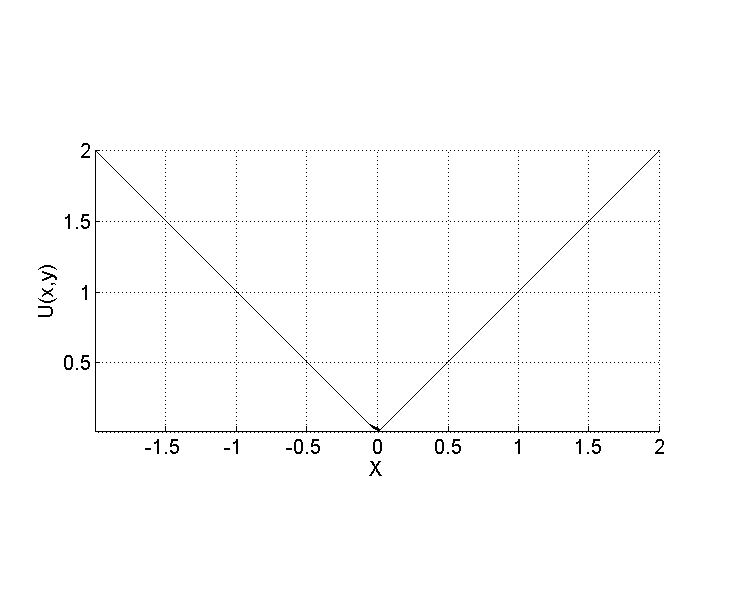
\includegraphics[width=\MeshFigWidth]{a02e01plot_XZ.png} 
		\caption{X-U Plane}
		\label{fig:a02e01plot_XZ}
	\end{subfigure}
	\vfill
	\begin{subfigure}{0.5\hsize}
		\centering
		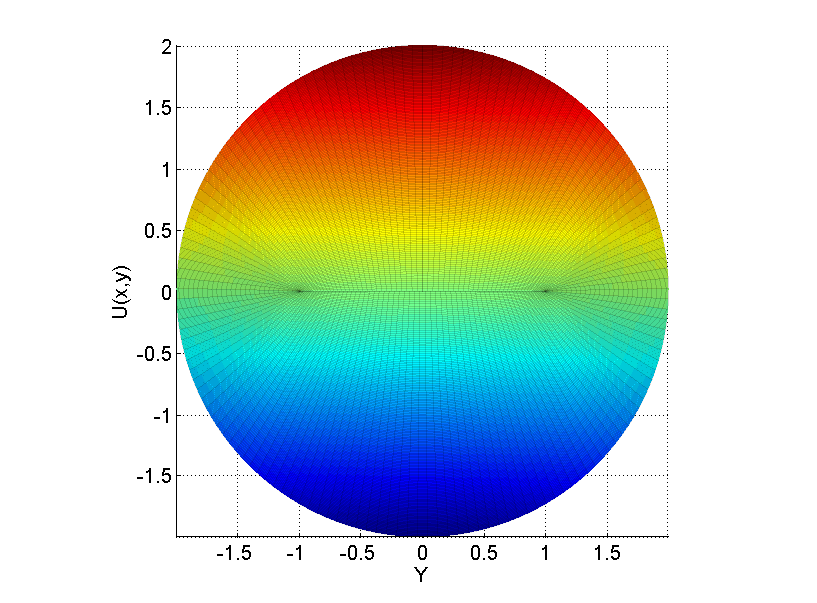
\includegraphics[width=\MeshFigWidth]{a02e01plot_YZ.png} 
		\caption{Y-U Plane}
		\label{fig:a02e01plot_YZ}
	\end{subfigure}
	\begin{subfigure}{0.5\hsize}
		\centering
		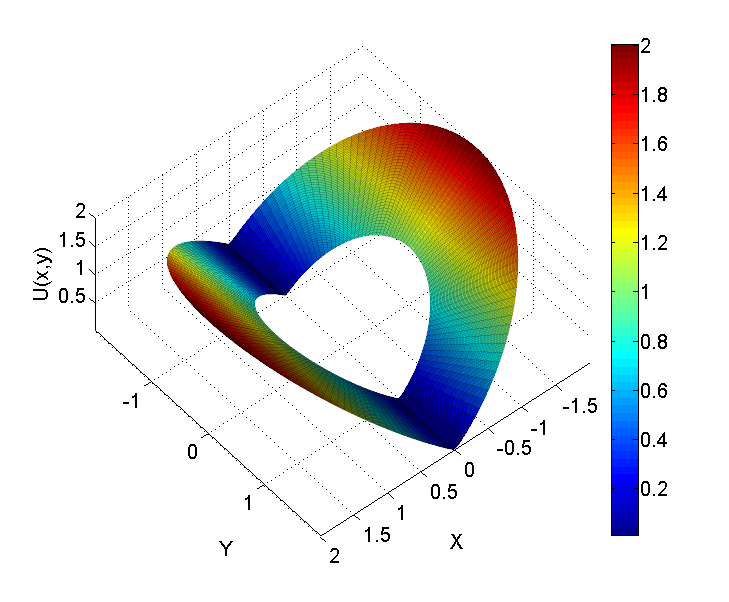
\includegraphics[width=\MeshFigWidth]{a02e01plot_Iso.png} 
		\caption{Isometric View}
		\label{fig:a02e01plot_Iso}
	\end{subfigure}
	\caption{Surface Plot of the Solution}
	\label{fig:a02e01plot}
\end{figure}

% EXERCISE 2
% --------------------------------------------------------------------------------------------------------------------
\addExercise{2}{Ex2}
%
% ----------------
%\addSubExercise{a}

%
% ----------------
%\addSubExercise{b}

%
% ----------------
%\addSubExercise{c}